\chapter{Results}
\label{cha:results}

This chapter presents the empirical results of evaluating the Trinity
architecture on Apple~Inc.\ (AAPL) daily equity data. All results reported
here are measured on the held-out test split (H2~2024, 116~trading days)
unless otherwise noted. Four system configurations are compared---Trinity
(the full architecture with C-Gate and Guardian), Executor-Only (the PPO
agent acting alone), Analyst-Only (the LLM agent acting alone), and
Trinity-no-CGate (a variant that bypasses the Consistency Gate and applies
the Guardian's adaptive policy using a naive agreement heuristic). Each
configuration that involves the Executor is evaluated across four frozen
random seeds (123, 4444, 6789, 9999); aggregate results report the mean
across these seeds, with per-seed breakdowns deferred to
Appendix~\ref{app:per-seed-results}. The chapter is organised as follows:
Section~\ref{sec:calibration} reports the C-Gate calibration output and
regime distribution; Section~\ref{sec:baselines} establishes baseline
performance under clean (non-adversarial) conditions;
Section~\ref{sec:adversarial} presents robustness under two adversarial
attack types; Section~\ref{sec:ablation} isolates the contribution of the
Consistency Gate through ablation; and Section~\ref{sec:results-summary}
summarises the findings against the sub-research questions. Results are
presented factually without interpretation; discussion and implications
follow in Chapter~\ref{cha:discussion}.

\section{C-Gate Calibration and Regime Distribution}
\label{sec:calibration}

The Consistency Gate was calibrated on the validation split
(2023-01-01--2024-06-30, 452~trading days) using the procedure described in
Section~\ref{sec:cgate}. Table~\ref{tab:calibration} summarises the
calibration output. The divergence metric $\Delta_t = 1 - \pi_{\text{RL}}
(d_{\text{LLM}} \mid s_t)$ was computed at temperature $T = 1.0$ (raw
softmax probabilities), yielding a validation-set mean of $0.735$ with
standard deviation $0.310$ and median $0.873$. The rightward skew of the
distribution---the median exceeds the mean by approximately $0.14$---reflects
the fact that the Executor's learned policy frequently assigns low
probability to the Analyst's recommended action, producing high divergence
values.

\begin{table}[h]
\centering
\caption{C-Gate calibration output on the validation split (452~samples,
  $T = 1.0$).}
\label{tab:calibration}
\begin{tabular}{ll}
\toprule
\textsc{Parameter} & \textsc{Value} \\
\midrule
$\tau_{\text{low}}$ (30th percentile)  & 0.6935 \\
$\tau_{\text{high}}$ (80th percentile) & 0.9877 \\
$\Delta$ mean / std                    & 0.735 / 0.310 \\
$\Delta$ median                        & 0.873 \\
$\Delta$ 10th / 90th percentile        & 0.153 / 0.997 \\
Agreement ($\Delta \leq \tau_{\text{low}}$) & 30.1\% \\
Ambiguity ($\tau_{\text{low}} < \Delta \leq \tau_{\text{high}}$) & 49.8\% \\
Conflict ($\Delta > \tau_{\text{high}}$) & 20.1\% \\
\bottomrule
\end{tabular}
\end{table}

The calibrated thresholds $\tau_{\text{low}} = 0.6935$ and $\tau_{\text{high}}
= 0.9877$ partition the validation set into three regimes: roughly 30\%
agreement, 50\% ambiguity, and 20\% conflict. Figure~\ref{fig:delta-hist}
shows the validation-set $\Delta$ distribution with the two threshold lines
overlaid.

\begin{figure}[h]
\centering
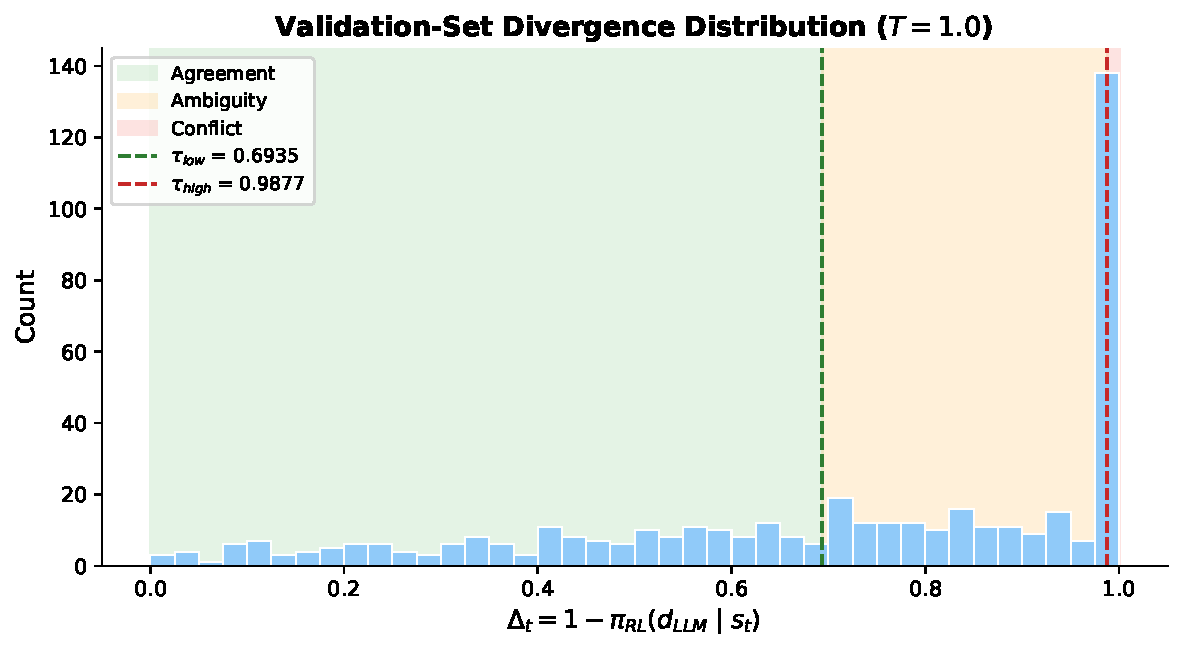
\includegraphics[width=0.85\textwidth]{figures/delta_histogram.pdf}
\caption{Distribution of the divergence metric $\Delta_t$ on the validation
  split (452~samples). Vertical dashed lines mark $\tau_{\text{low}} =
  0.6935$ and $\tau_{\text{high}} = 0.9877$. The three shaded regions
  correspond to the agreement, ambiguity, and conflict regimes.}
\label{fig:delta-hist}
\end{figure}

Table~\ref{tab:regime-test} reports the regime distribution on the test split
for each frozen seed. The distributions vary considerably across seeds: seed
9999, which has the highest entropy ratio among the frozen seeds (0.831),
produces a near-majority of agreement observations (53.4\%) and almost no
conflict (2.6\%), because its relatively flat policy distribution keeps
$\Delta$ values low. By contrast, seeds 123 and 4444---whose policies are
more sharply peaked (entropy ratios 0.321 and 0.299,
respectively)---generate conflict on roughly one-third of trading days.

\begin{table}[h]
\centering
\caption{C-Gate regime distribution on the test split, per seed.}
\label{tab:regime-test}
\begin{tabular}{lccc}
\toprule
\textsc{Seed} & \textsc{Agreement} & \textsc{Ambiguity} &
  \textsc{Conflict} \\
\midrule
123  & 15.5\% & 52.6\% & 31.9\% \\
4444 & 16.4\% & 44.8\% & 38.8\% \\
6789 & 25.9\% & 52.6\% & 21.6\% \\
9999 & 53.4\% & 44.0\% &  2.6\% \\
\bottomrule
\end{tabular}
\end{table}

\paragraph{Effect of temperature on calibration.}
An earlier calibration at $T = 0.05$ produced degenerate thresholds
($\tau_{\text{low}} = 0.9999$, $\tau_{\text{high}} = 1.0000$), because the
sharpened softmax collapsed the policy distribution to near-one-hot vectors,
pushing $\Delta$ to a bimodal $\{0, 1\}$ distribution with no continuous
middle range. Switching to $T = 1.0$ restored a continuous $\Delta$
distribution and improved mean test Sharpe from $-0.618$ to $-0.270$, while
mean test maximum drawdown decreased from $8.84\%$ to $8.60\%$. The
remaining temperature analysis is deferred to Chapter~\ref{cha:discussion}.

\section{Baseline Performance Under Clean Conditions}
\label{sec:baselines}

Before introducing adversarial perturbations, each configuration was
evaluated on the test split under clean (unmodified) market data and
signals. Table~\ref{tab:clean-baselines} reports the mean performance
metrics across the four frozen seeds. The Analyst-Only configuration has no
seed variation because the precomputed GPT-5 signals are deterministic;
its row reports a single run.

\begin{table}[h]
\centering
\caption{Mean test-split performance under clean conditions ($\pm$ denotes
  standard deviation across four seeds where applicable).}
\label{tab:clean-baselines}
\begin{tabular}{lrrrr}
\toprule
\textsc{Configuration} & \textsc{Sharpe} & \textsc{Sortino} &
  \textsc{Return (\%)} & \textsc{MaxDD (\%)} \\
\midrule
Trinity           & $-0.270$ & $-0.184$ & $-1.56$ & $\mathbf{8.60}$ \\
Executor-Only     & $-0.185$ & $-0.230$ & $-2.49$ & $15.28$ \\
Analyst-Only      & $-0.068$ & $-0.089$ & $-0.83$ & $9.12$ \\
Trinity-no-CGate  & $+0.238$ & $+0.425$ & $+0.92$ & $9.05$ \\
\bottomrule
\end{tabular}
\end{table}

Several observations follow from Table~\ref{tab:clean-baselines}. First,
Trinity achieves the lowest mean maximum drawdown at $8.60\%$, representing
a $44\%$ reduction relative to the Executor-Only baseline ($15.28\%$).
Second, none of the four configurations achieves a positive mean Sharpe
ratio except Trinity-no-CGate ($+0.238$), indicating that the test period
(H2~2024) is challenging for the trained policies. Third, the
Executor-Only configuration exhibits the highest drawdown by a wide
margin, approximately $1.8\times$ that of the next-worst configuration
(Analyst-Only at $9.12\%$). Fourth, the Analyst-Only configuration
produces the least negative mean Sharpe ($-0.068$) but cannot be directly
compared to seeded configurations because it involves a single
deterministic run.

Figure~\ref{fig:clean-maxdd} shows the mean maximum drawdown for each
configuration under clean conditions.

\begin{figure}[h]
\centering
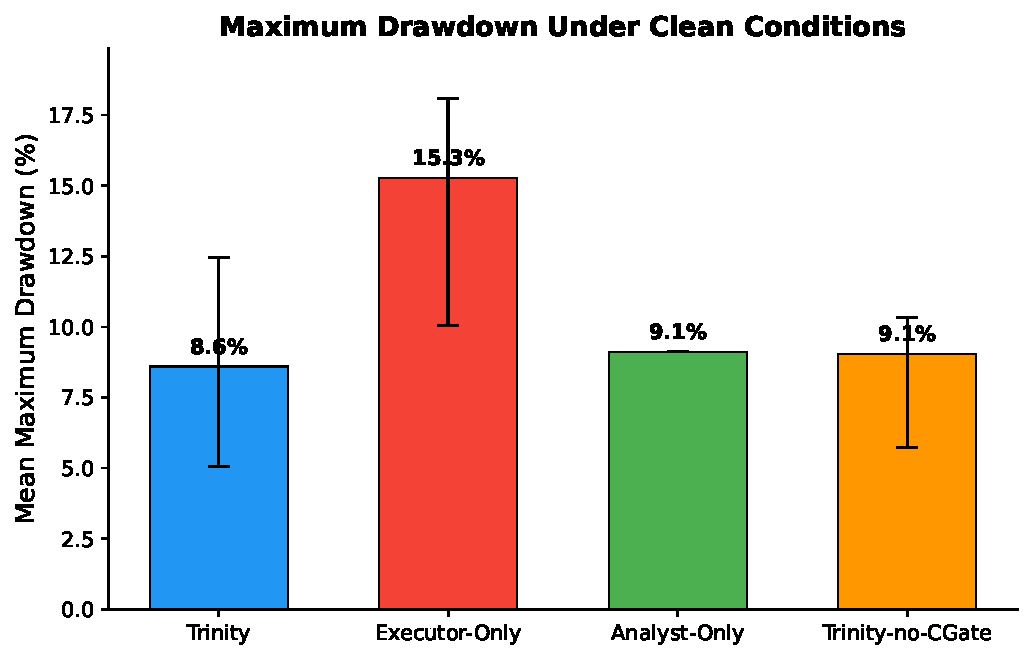
\includegraphics[width=0.7\textwidth]{figures/clean_maxdd_bar.pdf}
\caption{Mean maximum drawdown under clean conditions for each
  configuration. Error bars indicate the range across four seeds
  (omitted for Analyst-Only, which is a single deterministic run).}
\label{fig:clean-maxdd}
\end{figure}

The individual seed results exhibit substantial variation. Seed~123
achieves a Trinity Sharpe ratio of $+1.240$---the strongest individual
result across all configurations and seeds---while seed~6789 produces
$-2.079$. This cross-seed variance is typical of RL agents trained on
limited financial data and motivates the multi-seed evaluation design
described in Section~\ref{sec:eval-setup}. Per-seed breakdowns for all
configurations are provided in Appendix~\ref{app:per-seed-results}.

\section{Adversarial Robustness}
\label{sec:adversarial}

This section evaluates each configuration under two adversarial attack
types that target different channels of the Trinity architecture. Analyst
poisoning (Section~\ref{sec:analyst-poison}) corrupts the semantic channel
by flipping the Analyst's buy and sell signals. Executor perturbation
(Section~\ref{sec:executor-perturb}) corrupts the numeric channel by
injecting Gaussian noise into the Executor's observation vector. In both
cases, the attack is applied at five intensity levels to trace how
performance degrades as adversarial pressure increases.

% ------------------------------------------------------------------
\subsection{Analyst Poisoning}
\label{sec:analyst-poison}

Analyst poisoning randomly selects a fraction $r \in \{0.1, 0.2, 0.3,
0.4, 0.5\}$ of the Analyst's precomputed signals and flips their
directional component: buy becomes sell and vice versa, while hold signals
are left unchanged. This attack simulates a compromised or manipulated
language-model pipeline that injects adversarial trade recommendations.

Table~\ref{tab:poison-maxdd} reports the mean maximum drawdown across
four seeds for each configuration at each corruption rate.
Table~\ref{tab:poison-sharpe} reports the corresponding mean Sharpe
ratios.

\begin{table}[h]
\centering
\caption{Mean maximum drawdown (\%) under analyst poisoning, by corruption
  rate and configuration. Bold marks the lowest (best) MaxDD in each row.}
\label{tab:poison-maxdd}
\begin{tabular}{lcccc}
\toprule
\textsc{Rate} & \textsc{Trinity} & \textsc{Executor-Only} &
  \textsc{Analyst-Only} & \textsc{Trinity-no-CGate} \\
\midrule
10\% & \textbf{8.60} & 15.28 &  9.21 &  9.05 \\
20\% & 9.98           & 15.28 & 12.09 & \textbf{9.05} \\
30\% & \textbf{7.15}  & 15.28 &  4.23 &  8.16 \\
40\% & \textbf{7.55}  & 15.28 &  6.62 &  8.71 \\
50\% & \textbf{8.80}  & 15.28 & 12.18 & 10.29 \\
\bottomrule
\end{tabular}
\end{table}

\begin{table}[h]
\centering
\caption{Mean Sharpe ratio under analyst poisoning, by corruption rate and
  configuration.}
\label{tab:poison-sharpe}
\begin{tabular}{lcccc}
\toprule
\textsc{Rate} & \textsc{Trinity} & \textsc{Executor-Only} &
  \textsc{Analyst-Only} & \textsc{Trinity-no-CGate} \\
\midrule
10\% & $-0.198$ & $-0.185$ & $-0.084$ & $+0.235$ \\
20\% & $-1.039$ & $-0.185$ & $-1.544$ & $-0.207$ \\
30\% & $+0.834$ & $-0.185$ & $+1.738$ & $+0.626$ \\
40\% & $-0.144$ & $-0.185$ & $+0.176$ & $+0.283$ \\
50\% & $+0.030$ & $-0.185$ & $-0.864$ & $-0.011$ \\
\bottomrule
\end{tabular}
\end{table}

Three patterns emerge from Tables~\ref{tab:poison-maxdd}
and~\ref{tab:poison-sharpe}. First, Trinity's mean MaxDD remains within a
narrow band of $7.15\%$--$9.98\%$ across all five corruption rates---a
total range of $2.83$~percentage points (pp). This is the tightest MaxDD
band among the multi-agent configurations. Second, the Executor-Only
configuration is entirely unaffected by analyst poisoning because the
Executor receives no analyst signals by design; its MaxDD remains
constant at $15.28\%$ across all rates, confirming the channel
independence property of the architecture. Third, the Analyst-Only
configuration exhibits the widest MaxDD variation ($4.23\%$--$12.18\%$,
a range of $7.95$~pp), because it directly consumes the poisoned signals
without any gating or filtering mechanism. The anomalously low MaxDD at
the $30\%$ corruption rate ($4.23\%$) indicates that the particular
random subset of flipped signals happened to improve alignment with
realised market movements during the test period---an artefact of the
single-run, single-asset evaluation rather than a systematic effect.

Figure~\ref{fig:poison-maxdd} visualises the MaxDD trajectories across
corruption rates.

\begin{figure}[h]
\centering
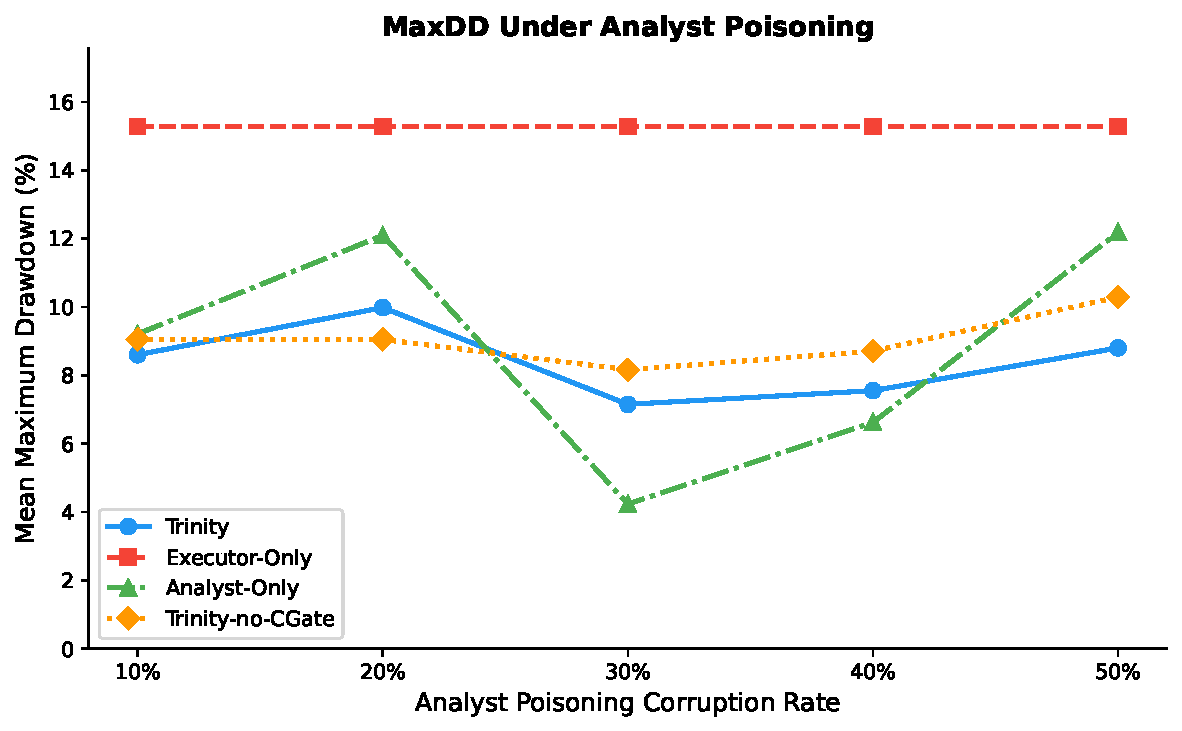
\includegraphics[width=0.85\textwidth]{figures/analyst_poison_maxdd.pdf}
\caption{Mean maximum drawdown vs.\ analyst poisoning corruption rate for
  each configuration. The shaded band around each line indicates the range
  across four seeds (omitted for Analyst-Only and Executor-Only, which have
  no seed variation under this attack).}
\label{fig:poison-maxdd}
\end{figure}

% ------------------------------------------------------------------
\subsection{Executor Perturbation}
\label{sec:executor-perturb}

Executor perturbation injects additive Gaussian noise $\mathcal{N}(0,
\sigma)$ into the Executor's z-normalised observation vector at each
timestep, with $\sigma \in \{0.1, 0.2, 0.3, 0.4, 0.5\}$. Because the
observations are z-normalised to approximately unit variance, a
perturbation of $\sigma = 0.5$ represents noise at half the scale of the
signal itself---a substantial corruption of the numeric channel.

Table~\ref{tab:perturb-maxdd} reports the mean maximum drawdown and
Table~\ref{tab:perturb-sharpe} reports the mean Sharpe ratio for each
configuration at each noise level.

\begin{table}[h]
\centering
\caption{Mean maximum drawdown (\%) under executor perturbation, by noise
  level $\sigma$ and configuration. Bold marks the lowest MaxDD in each
  row.}
\label{tab:perturb-maxdd}
\begin{tabular}{lcccc}
\toprule
$\sigma$ & \textsc{Trinity} & \textsc{Executor-Only} &
  \textsc{Analyst-Only} & \textsc{Trinity-no-CGate} \\
\midrule
0.1 & 9.19           & 15.76 & 9.12           & \textbf{8.81} \\
0.2 & 7.98           & 14.58 & 9.12           & \textbf{8.67} \\
0.3 & \textbf{6.89}  & 14.35 & 9.12           & 8.36 \\
0.4 & \textbf{7.19}  & 13.74 & 9.12           & 8.04 \\
0.5 & \textbf{6.23}  & 11.28 & 9.12           & 6.56 \\
\bottomrule
\end{tabular}
\end{table}

\begin{table}[h]
\centering
\caption{Mean Sharpe ratio under executor perturbation, by noise level
  $\sigma$ and configuration.}
\label{tab:perturb-sharpe}
\begin{tabular}{lcccc}
\toprule
$\sigma$ & \textsc{Trinity} & \textsc{Executor-Only} &
  \textsc{Analyst-Only} & \textsc{Trinity-no-CGate} \\
\midrule
0.1 & $-0.947$ & $-0.304$ & $-0.068$ & $+0.227$ \\
0.2 & $+0.234$ & $-0.381$ & $-0.068$ & $+0.008$ \\
0.3 & $+0.866$ & $+0.573$ & $-0.068$ & $+0.997$ \\
0.4 & $-0.191$ & $+0.029$ & $-0.068$ & $+0.390$ \\
0.5 & $+0.557$ & $+0.894$ & $-0.068$ & $+1.251$ \\
\bottomrule
\end{tabular}
\end{table}

The results exhibit a pattern that mirrors the analyst-poisoning
experiment along the opposite channel. First, Trinity's mean MaxDD
ranges from $6.23\%$ to $9.19\%$---a band of $2.96$~pp---again the
tightest among the seeded configurations. Second, the Analyst-Only
configuration is entirely unaffected ($9.12\%$ constant), confirming
channel independence in the reverse direction: perturbation of the
numeric channel does not propagate to the semantic channel. Third, the
Executor-Only configuration starts at the highest MaxDD ($15.76\%$ at
$\sigma = 0.1$) and decreases to $11.28\%$ at $\sigma = 0.5$. This
counter-intuitive improvement at high noise levels likely reflects
the noise inadvertently diversifying the Executor's action selection
on a test period where its learned policy performs poorly.

Figure~\ref{fig:perturb-maxdd} visualises the MaxDD trajectories under
executor perturbation.

\begin{figure}[h]
\centering
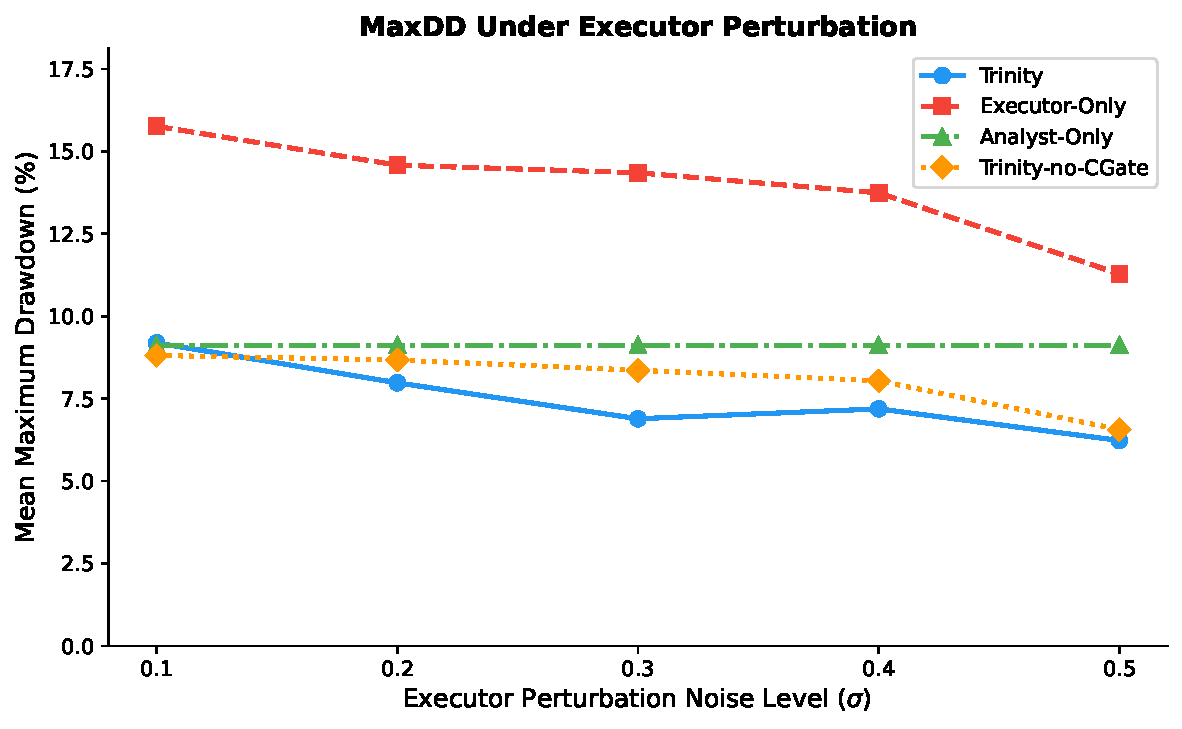
\includegraphics[width=0.85\textwidth]{figures/executor_perturb_maxdd.pdf}
\caption{Mean maximum drawdown vs.\ executor perturbation noise level
  $\sigma$ for each configuration. The shaded band around each line
  indicates the range across four seeds (omitted for Analyst-Only, which
  has no seed variation under this attack).}
\label{fig:perturb-maxdd}
\end{figure}

\paragraph{Cross-attack summary.}
Across both attack types and all ten attack intensities, Trinity's mean
maximum drawdown stays within a combined range of $6.23\%$--$9.98\%$. By
comparison, the Executor-Only configuration ranges from $11.28\%$ to
$15.76\%$ and the Analyst-Only configuration ranges from $4.23\%$ to
$12.18\%$. Trinity thus exhibits the most stable drawdown profile among
all configurations that are exposed to adversarial pressure on their
respective input channels.

\section{Ablation: Contribution of the Consistency Gate}
\label{sec:ablation}

The Trinity-no-CGate configuration removes the Consistency Gate and instead
applies the Guardian's adaptive policy using a naive heuristic: if the
Analyst and Executor agree on the same discrete action the system treats
the situation as agreement; otherwise it treats it as ambiguity. This
ablation isolates the C-Gate's contribution by holding all other
components (Executor, Analyst, Guardian) constant.

Table~\ref{tab:ablation} compares Trinity and Trinity-no-CGate across
three evaluation conditions: clean (no attack), analyst poisoning (mean
across all five corruption rates), and executor perturbation (mean across
all five noise levels).

\begin{table}[h]
\centering
\caption{Trinity vs.\ Trinity-no-CGate: mean maximum drawdown (\%) across
  evaluation conditions. $\Delta_{\text{pp}}$ denotes the difference in
  percentage points (negative means Trinity is lower).}
\label{tab:ablation}
\begin{tabular}{lccc}
\toprule
\textsc{Condition} & \textsc{Trinity} & \textsc{Trinity-no-CGate} &
  $\Delta_{\text{pp}}$ \\
\midrule
Clean                              & 8.60 & 9.05 & $-0.45$ \\
Analyst poisoning (mean of 5 rates) & 8.42 & 9.05 & $-0.63$ \\
Executor perturbation (mean of 5 $\sigma$) & 7.50 & 8.09 & $-0.59$ \\
\midrule
Overall (all conditions)           & 8.04 & 8.60 & $-0.56$ \\
\bottomrule
\end{tabular}
\end{table}

The results in Table~\ref{tab:ablation} show that Trinity achieves lower
mean MaxDD than Trinity-no-CGate in every condition. The improvement is
modest---between $0.45$ and $0.63$~pp---but consistent across all three
evaluation settings. Under analyst poisoning, the C-Gate's continuous
divergence metric allows the system to modulate its response proportionally
to the degree of agent disagreement, rather than relying on a binary
agree/disagree heuristic. Under executor perturbation, the C-Gate detects
when the Executor's corrupted observations produce policy distributions
that diverge from the Analyst's recommendation, triggering position
scaling or fail-safe responses.

Table~\ref{tab:ablation-sharpe} presents the corresponding Sharpe ratio
comparison. Trinity-no-CGate achieves higher mean Sharpe than Trinity in
every condition, indicating that the C-Gate's conservative regime
policy---particularly the conflict-regime fail-safe to flat---sacrifices
return in exchange for drawdown reduction.

\begin{table}[h]
\centering
\caption{Trinity vs.\ Trinity-no-CGate: mean Sharpe ratio across
  evaluation conditions.}
\label{tab:ablation-sharpe}
\begin{tabular}{lcc}
\toprule
\textsc{Condition} & \textsc{Trinity} & \textsc{Trinity-no-CGate} \\
\midrule
Clean                              & $-0.270$ & $+0.238$ \\
Analyst poisoning (mean of 5 rates) & $-0.103$ & $+0.185$ \\
Executor perturbation (mean of 5 $\sigma$) & $+0.104$ & $+0.575$ \\
\bottomrule
\end{tabular}
\end{table}

The ablation also provides indirect evidence for the channel-independence
property central to SRQ1. Under analyst poisoning, the Executor-Only
configuration is entirely unaffected (constant MaxDD of $15.28\%$ across
all corruption rates), confirming that compromise of the semantic channel
does not propagate to the numeric channel. Symmetrically, under executor
perturbation the Analyst-Only configuration remains constant at $9.12\%$
MaxDD. This bidirectional isolation is a direct consequence of the
architectural separation described in Section~\ref{sec:architecture}: the
Analyst observes only text headlines and the Executor observes only
numeric features, with no shared inputs or intermediate representations.

\section{Summary of Results}
\label{sec:results-summary}

Table~\ref{tab:results-summary} maps each sub-research question to the
principal empirical findings reported in this chapter.

\begin{table}[h]
\centering
\caption{Summary of empirical findings by sub-research question.}
\label{tab:results-summary}
\begin{tabular}{p{1.2cm}p{5cm}p{6.5cm}}
\toprule
\textsc{SRQ} & \textsc{Question (abbreviated)} & \textsc{Key Finding} \\
\midrule
SRQ1 &
  Component decomposition and correlated-failure reduction &
  Channel independence confirmed: analyst poisoning leaves Executor-Only
  metrics unchanged across all five corruption rates; executor
  perturbation leaves Analyst-Only metrics unchanged across all five
  noise levels. Compromise of one channel does not propagate to the
  other. \\
\addlinespace
SRQ2 &
  Cross-modal divergence definition and calibration &
  $\Delta_t = 1 - \pi_{\text{RL}}(d_{\text{LLM}} \mid s_t)$ calibrated
  at $T = 1.0$ with data-driven thresholds $\tau_{\text{low}} = 0.6935$,
  $\tau_{\text{high}} = 0.9877$, yielding a $30/50/20$ regime split on
  validation data with meaningful per-seed variation on the test split. An
  earlier calibration at $T = 0.05$ produced degenerate thresholds,
  confirming that temperature selection is critical for the metric's
  discriminative power. \\
\addlinespace
SRQ3 &
  Measurable robustness improvement under adversarial conditions &
  Trinity reduces mean MaxDD by $44\%$ relative to Executor-Only under
  clean conditions ($8.60\%$ vs.\ $15.28\%$). Under adversarial
  pressure, Trinity's mean MaxDD remains within $6.23\%$--$9.98\%$
  across all ten attack intensities, compared to $11.28\%$--$15.76\%$
  for Executor-Only. The C-Gate contributes a consistent
  $0.45$--$0.63$~pp MaxDD reduction over the Trinity-no-CGate ablation.
  \\
\bottomrule
\end{tabular}
\end{table}


% \chapter{Results} \label{cha:results}

% In the Results part of the thesis, you objectively present the results of your study without interpreting them or discussing their wider implications. You answer the research question by presenting your quantitative or qualitative analysis outcomes. And you convey your data and
% other results through text, tables, figures, and other visual means.

% Tables are often helpful for presenting results. For example, have a look at Table \ref{tab:titles1}.

% \begin {table} [h]
% \begin{tabular}{ccc}
% \hline
% \textsc{Author} & \textsc{Title} & \textsc{Year}\\
% \hline
% \verb|Gottlob Frege| & \verb|Begriffsschrift| & \rmfamily 1879
% \\
% \verb|Bertrand Russell| & \verb|Principia Mathematica| & \sffamily 1910
% \\
% \verb|Ludwig Wittgenstein| & \verb|Philosophical Investigations| & \ttfamily 1953\\
% \hline
% \end{tabular}
% \caption {Philosophical Titles 1} \label{tab:titles1} 
% \end{table}

% The same data are shown in Table \ref{tab:titles2} but with different formatting.

% \begin {table} [h] 
% \begin{tabular}{lll}
% \toprule[1.5pt]
% \textsc{Author} & \textsc{Title} & \textsc{Year}\\
% \midrule
% \verb|Gottlob Frege| & \verb|Begriffsschrift| & \rmfamily 1879
% \\
% \verb|Bertrand Russell| & \verb|Principia Mathematica| & \sffamily 1910
% \\
% \verb|Ludwig Wittgenstein| & \verb|Philosophical Investigations| & \ttfamily 1953\\
% \bottomrule[1.5pt] 
% \end{tabular}
% \caption {Philosophical Titles 2} \label{tab:titles2}
% \end{table}

% The table tool in Overleaf can be handy for inserting and managing tables.